\documentclass{article}

\usepackage{amsmath,amssymb}
\usepackage{tikz}
\usepackage{pgfplots}
\usepackage{xcolor}
\usepackage[left=2.1cm,right=3.1cm,bottom=3cm,footskip=0.75cm,headsep=0.5cm]{geometry}
\usepackage{enumerate}
\usepackage{enumitem}
\usepackage{marvosym}
\usepackage{tabularx}
\usepackage[amsmath,thmmarks,standard]{ntheorem}
\usepackage{mathtools}

\usepackage[utf8]{inputenc}

\renewcommand*{\arraystretch}{1.4}
\newcommand{\E}{\mathbb{E}}

\newcolumntype{L}[1]{>{\raggedright\arraybackslash}p{#1}}
\newcolumntype{R}[1]{>{\raggedleft\arraybackslash}p{#1}}
\newcolumntype{C}[1]{>{\centering\let\newline\\\arraybackslash\hspace{0pt}}m{#1}}

\DeclareMathOperator{\tr}{tr}
\DeclareMathOperator{\Var}{Var}
\DeclareMathOperator{\Cov}{Cov}
\renewcommand{\E}{\mathbb{E}}

\newtheorem{thm}{Theorem}
\newtheorem{lem}{Lemma}

\title{\textbf{Einführung in die Logistik, Übung 3}}
\author{\textsc{Henry Haustein}}
\date{}

\begin{document}
	\maketitle
	
	\section*{Aufgabe 6}
	\begin{enumerate}[label=(\alph*)]
		\item Graph
		\begin{center}
			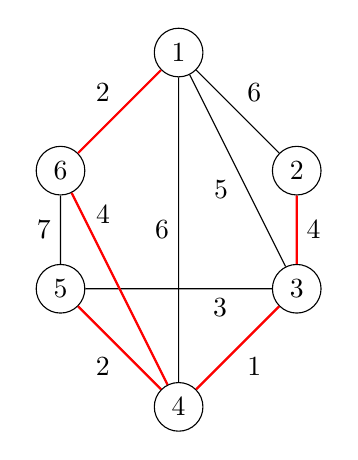
\begin{tikzpicture}
				\node[circle,draw=black, fill=white] (1) at (0,0) {1};
				\node[circle,draw=black, fill=white] (2) at (1.5,-1.5) {2};
				\node[circle,draw=black, fill=white] (3) at (1.5,-3) {3};
				\node[circle,draw=black, fill=white] (4) at (0,-4.5) {4};
				\node[circle,draw=black, fill=white] (5) at (-1.5,-3) {5};
				\node[circle,draw=black, fill=white] (6) at (-1.5,-1.5) {6};
				
				\draw (1) to node[above right] {6} (2) to node[right] {4} (3) to node[below right] {1} (4) to node[below left] {2} (5) to node[left] {7} (6) to node[above left] {2} (1);
				\draw (1) to node[below left] {5} (3) to node[below,xshift=15] {3} (5);
				\draw (1) to node[left] {6} (4) to node[above right,xshift=-12,yshift=20] {4} (6);
				
				\draw[red,thick] (2) -- (3) -- (4) -- (6) -- (1);
				\draw[red,thick] (4) -- (5);
			\end{tikzpicture}
		\end{center}
		\item Algorithmus von Prim
		\begin{itemize}
			\item $W=\{3\}$, $V=\{1,2,4,5,6\}$, $E^\ast=\{[3,4]\}$, $W=\{3,4\}$, $V=\{1,2,5,6\}$
			\item wähle $[4,5]$: $E^\ast=\{[3,4],[4,5]\}$, $W=\{3,4,5\}$, $V=\{1,2,6\}$
			\item wähle $[4,6]$: $E^\ast=\{[3,4],[4,5],[4,6]\}$, $W=\{3,4,5,6\}$, $V=\{1,2\}$
			\item wähle $[6,1]$: $E^\ast=\{[3,4],[4,5],[4,6],[6,1]\}$, $W=\{1,3,4,5,6\}$, $V=\{2\}$
			\item wähle $[3,2]$: $E^\ast=\{[3,4],[4,5],[4,6],[6,1],[3,2]\}$, $W=\{1,2,3,4,5,6\}$, $V=\emptyset \Rightarrow$ Ende
		\end{itemize}
	\end{enumerate}

	\section*{Aufgabe 7}
	Es gibt eine sehr schöne Schreibweise für den Ablauf des Algorithmus aus der Vorlesung \textit{Einführung in die Informatik}. Dabei ist die Menge $S$ die Menge der bisher erkundeten Punkte, zu diesen Punkten kennt man den kürzesten Weg und $D(i)$ ist die (kumulierte) Distanz zum Knoten $i$. Die \underline{unterstrichene} Distanz ist die kürzeste Distanz zu einem noch nicht erkundeten Punkt
	\begin{center}
		\begin{tabular}{c|c|ccccc}
			Iteration & $S$ & $D(1)$ & $D(2)$ & $D(3)$ & $D(5)$ & $D(6)$ \\
			\hline
			0 & $\{4\}$ & $\infty$ & 4 & 6 & \underline{2} & $\infty$ \\
			1 & $\{4,5\}$ & $\infty$ & \underline{4} & 6 & 2 & $\infty$ \\
			2 & $\{2,4,5\}$ & \underline{6} & 4 & 6 & 2 & $\infty$ \\
			3 & $\{1,2,4,5\}$ & 6 & 4 & \underline{6} & 2 & 7 \\
			4 & $\{1,2,3,4,5\}$ & 6 & 4 & 6 & 2 & \underline{7} \\
			5 & $\{1,2,3,4,5,6\}$ & 6 & 4 & 6 & 2 & 7
		\end{tabular}
	\end{center}
	
	\section*{Aufgabe 8}
	\begin{enumerate}[label=(\alph*)]
		\item Die Bewertungsmatrix lautet
		\begin{align}
			C(\vec{G}) = \begin{array}{c|cccccc}
			& 1 & 2 & 3 & 4 & 5 & 6 \\
			\hline
			1 & 0 & 340 & 530 & \infty & \infty & \infty \\
			2 & \infty & 0 & 280 & 750 & \infty & \infty \\
			3 & \infty & \infty & 0 & 570 & 480 & \infty \\
			4 & \infty & \infty & \infty & 0 & 460 & 810 \\
			5 & \infty & \infty & \infty & \infty & 0 & 840 \\
			6 & \infty & \infty & \infty & \infty & \infty & 0
			\end{array} \notag
		\end{align}
		\item Anwendung des Verfahrens von Bellmann liefert
		\begin{center}
			\begin{tabular}{c|c|c}
				$j$ & $d_{1j}$ & $V(j)$ \\
				\hline
				1 & 0 & 1 \\
				2 & 340 & 1 \\
				3 & 530 & 1 \\
				4 & 1090 & 2 \\
				5 & 1100 & 3 \\
				6 & 1900 & 4
			\end{tabular}
		\end{center}
		\item Arbeitet man die Tabelle von unten nach oben durch, so ergibt sich 6 $\leftarrow 4 \leftarrow 2 \leftarrow 1$, also ist der kürzeste Weg: $1 \to 2 \to 4 \to 6$.
		\item Baumalgorithmen ermitteln den kürzesten Weg von einem Startknoten zu allen anderen Knoten, z.B. Dijkstra-Algorithmus \\
		Matrixalgorithmen ermitteln den kürzesten Weg von jedem Knoten zu jedem Knoten, z.B. Tripelalgorithmus
	\end{enumerate}

	\section*{Aufgabe 9}
	\begin{enumerate}[label=(\alph*)]
		\item Graph
		\begin{center}
			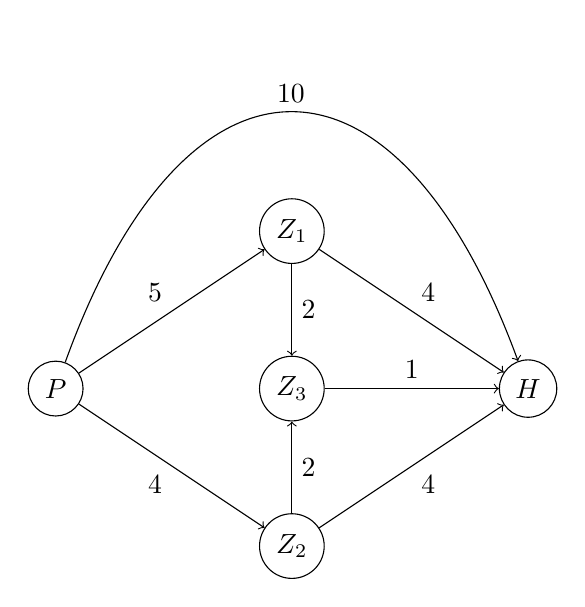
\begin{tikzpicture}
				\node[circle,draw=black, fill=white] (P) at (0,0) {$P$};
				\node[circle,draw=black, fill=white] (Z1) at (3,2) {$Z_1$};
				\node[circle,draw=black, fill=white] (Z2) at (3,-2) {$Z_2$};
				\node[circle,draw=black, fill=white] (Z3) at (3,0) {$Z_3$};
				\node[circle,draw=black, fill=white] (H) at (6,0) {$H$};
				
				\draw[->] (P) to[bend left=70,looseness=2] node[above] {10} (H);
				\draw[->] (P) to node[above left] {5} (Z1);
				\draw[->] (P) to node[below left] {4} (Z2);
				\draw[->] (Z1) to node[above right] {4} (H);
				\draw[->] (Z1) to node[right] {2} (Z3);
				\draw[->] (Z2) to node[below right] {4} (H);
				\draw[->] (Z2) to node[right] {2} (Z3);
				\draw[->] (Z3) to node[above] {1} (H);
			\end{tikzpicture}
		\end{center}
		Die Vorgängermatrix lautet
		\begin{align}
			\begin{array}{c|ccccc}
				W^0 & P & Z_1 & Z_2 & Z_3 & H \\
				\hline
				P & P & P & P & \infty & P \\
				Z_1 & \infty & Z_1 & \infty & Z_1 & Z_1 \\
				Z_2 & \infty & \infty & Z_2 & Z_2 & Z_2 \\
				Z_3 & \infty & \infty & \infty & Z_3 & Z_3 \\
				H & \infty & \infty & \infty & \infty & H
			\end{array} \notag
		\end{align}
		\item Die Entfernungsmatrix und die Wegematrix lauten
		\begin{align}
			\begin{array}{c|ccccc}
				D & P & Z_1 & Z_2 & Z_3 & H \\
				\hline
				P & 0 & 5 & 4 & 6 & 7 \\
				Z_1 & \infty & 0 & \infty & 2 & 4 \\
				Z_2 & \infty & \infty & 0 & 2 & 4 \\
				Z_3 & \infty & \infty & \infty & 0 & 1 \\
				H & \infty & \infty & \infty & \infty & 0
			\end{array} \quad
			 \begin{array}{c|ccccc}
			 	W & P & Z_1 & Z_2 & Z_3 & H \\
			 	\hline
			 	P & P & P & P & Z_2 & Z_2Z_3 \\
			 	Z_1 & \infty & Z_1 & \infty & Z_1 & Z_1 \\
			 	Z_2 & \infty & \infty & Z_2 & Z_2 & Z_2 \\
			 	Z_3 & \infty & \infty & \infty & Z_3 & Z_3 \\
			 	H & \infty & \infty & \infty & \infty & H
			 \end{array}\notag
		\end{align}
		Die Entfernungsmatrix gibt die Entfernung zwischen 2 Punkten an und die Wegematrix den Weg.
		\item Mit der selben Notation wie in Aufgabe 7 folgt
		\begin{center}
			\begin{tabular}{c|c|cccc}
				Iteration & $S$ & $D(Z_1)$ & $D(Z_2)$ & $D(Z_3)$ & $D(H)$ \\
				\hline
				0 & $\{P\}$ & 5 & \underline{4} & $\infty$ & 10 \\
				1 & $\{P,Z_2\}$ & \underline{5} & 4 & 6 & 8 \\
				2 & $\{P,Z_1,Z_2\}$ & 5 & 4 & \underline{6} & 8 \\
				3 & $\{P,Z_1,Z_2,Z_3\}$ & 5 & 4 & 6 & \underline{7} \\
				4 & $\{P,Z_1,Z_2,Z_3,H\}$ & 5 & 4 & 6 & 7
			\end{tabular}
		\end{center}
	\end{enumerate}
	
\end{document}